%!TEX options = --shell-escape
\documentclass[notitlepage,11pt]{report}
\usepackage[left=1in, right=1in, top=1in, bottom=1in]{geometry}
\usepackage{amssymb}
\usepackage{bondgraphs}
\usepackage{multicol}
\usepackage{titling}
\renewcommand{\abstractname}{\vspace{-\baselineskip}}

% \pretitle{\begin{center}\Huge\bfseries}
% \posttitle{\par\end{center}\vskip 0.5em}
% \preauthor{\begin{center}\Large\ttfamily}
% \postauthor{\end{center}}
% \predate{\par\large\centering}
% \postdate{\par}

\title{Modelling a Crankshaft-Magnetomotive Force System}
\author{Ramandeep Farmaha \\ Kush Thaker \\ Siddhanth Unnithan}
\date{\today}
\begin{document}

\maketitle
\thispagestyle{empty}

\begin{abstract}
Insert the Abstract hereInsert the Abstract hereInsert the Abstract hereInsert the Abstract hereInsert the Abstract hereInsert the Abstract hereInsert the Abstract hereInsert the Abstract hereInsert the Abstract hereInsert the Abstract hereInsert the Abstract hereInsert the Abstract hereInsert the Abstract here
\end{abstract}
\begin{multicols}{2}
The designed system consists of two components: an inertial wheel with a crankshaft arm attached, and a cart mass with a spring. Railings are used to constrain the wheel arm, cart and springs in the x direction. A pair of strong magnets are attached to the wheel arm and cart. As torque is applied to the wheel, the crankshaft arm moves towards the cart, and a magnetic force is applied to the second component of the system. The force causes the cart to flow towards the springs and rebound along the rail. The cart oscillates between the crankshaft arm and springs until the wheel stops rotating.

The prototype was constructed as a wooden body with metal and acrylic supports. It started with a large wooden wheel on one side which could be turned by the operator. On the other side, metal rods were installed as rails to align the direction of the crankshaft arm, cart and springs. The cart was simply a block of wood with screwed in eye bolts; the loops allowed for a sliding motion along the rails. The crankshaft used to convert rotational motion into linear motion was trickier to implement. The arm length had to be the correct length to allow for the wheel to rotate without interference, but also get close enough to the cart to push it into springs. It was ultimately implemented as an acrylic arm mounted on the inner radius of the wheel attached to another piece of acrylic sliding linearly along the rails. Finally, one magnet was glued to the crankshaft arm, while the other was placed on the cart.

A point to note about the physical prototype is that the human operated power source applied to the wheel was a quick adjustment made for demo-day. By manually giving the wheel an angular velocity, it is a source of flow that is applied, not a source of effort. However, a source of effort is required to avoid derivative causalities in the bond graph model. The preferable prototype implementation would have used a torsional spring or elastic band to wind up the wheel and give it torque, which would have been consistent with the bond graph.

There were also problems encountered in applying the theoretical system into practice. For one, the friction was too great along the rails, causing the crankshaft arm and cart to slide unsmoothly. Friction could have been reduced by using ball bearings to slide against the rails instead of simple holes and lubricant. Next, the springs were too stiff, limiting the cart’s rebound motion. A spring with a lesser k value could compress further and exert a greater rebound force on the cart. Thirdly, the strength of the magnets was too small to push the cart into the springs with enough force. Like decreasing the spring’s stiffness, a greater repelling force applied to the cart could also have created a preferred rebound motion. These problems together limited the cart from oscillating along the rail as desired.
% Initial bondgraph
\begin{figure*}
   \centering
   \tikzstyle{block}=[minimum width=7mm,minimum height=7mm,draw,thick]
   \tikzstyle{signal} = [-latex, color=red!30!black]
   \begin{tikzpicture}
      \node[bgelement, label=north:$mmf_i$$_n$] (Se) at (0,0) {SE};
      \node[bgelement] (one) at (2,0) {1};
      \node[bgelement, label=right:$\frac{1}{k}$] (C) at (4,0) {C};
      \node[bgelement, above=1 of one, label=north:$m_2$] (I) {I};
      \node[bgelement] (oneright) at (-3, 0) {1};
      \node[bgelement, above=1 of oneright, label=north:$m_1$] (Im1) {I};
      \node[bgelement, left=1 of oneright, label=south:R] (TF) {TF};
      \node[bgelement, left=1 of TF] (oneleft) {1};
      \node[bgelement, above=1 of oneleft, label=north:J] (IJ) {I};
      \node[bgelement, left=1 of oneleft, label=south:$T_i$$_n$] (SEin) {SE};
      \node[block,below=1 of TF] (int) {$\int$};
      \node[block,right=1 of int] (ddt) {$\theta$};
      \draw[bond,f_in] (Se) -- (one);
      \draw[bond, f_in] (one) -- (I);
      \draw[bond, f_out] (one) -- (C);
      \draw[bond, f_out={error}] (oneright) -- (Im1);
      \draw[bond, f_out] (TF) -- (oneright);
      \draw[bond, f_out] (oneleft) -- (TF);
      \draw[bond, f_in] (oneleft) -- (IJ);
      \draw[bond, f_in] (SEin) -- (oneleft);
      \begin{scope}[every path/.style={signal}]
      		\draw (oneleft) -- node[pos=0.5,right]{$w$} (int);
      		\draw (int) -- (ddt);
      		\draw (ddt) -- (Se);
      	\end{scope}
    \end{tikzpicture}
    \caption{Bondgraph modelling magnetomotive force as SE}
\end{figure*}
% Initial bondgraph
\begin{figure*}
   \centering
   \tikzstyle{block}=[minimum width=7mm,minimum height=7mm,draw,thick]
   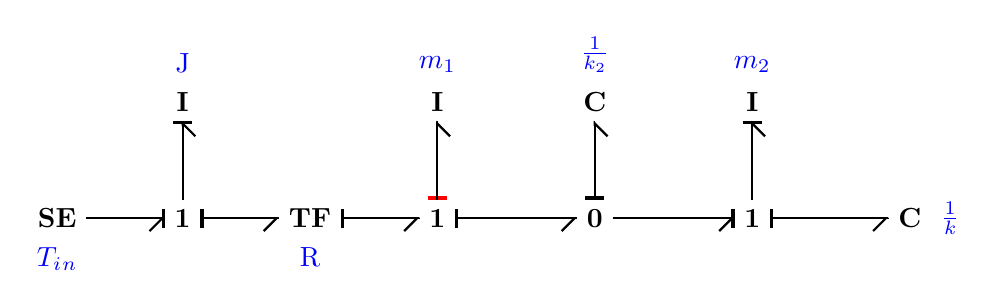
\begin{tikzpicture}
      \node[bgelement] (0bond) at (0,0) {0};
      \node[bgelement] (one) at (2,0) {1};
      \node[bgelement, label=right:$\frac{1}{k}$] (C) at (4,0) {C};
      \node[bgelement, above=1 of one, label=north:$m_2$] (I) {I};
      \node[bgelement] (oneright) at (-2, 0) {1};
      \node[bgelement, above=1 of oneright, label=north:$m_1$] (Im1) {I};
      \node[bgelement, left=1 of oneright, label=south:R] (TF) {TF};
      \node[bgelement, left=1 of TF] (oneleft) {1};
      \node[bgelement, above=1 of oneleft, label=north:J] (IJ) {I};
      \node[bgelement, left=1 of oneleft, label=south:$T_i$$_n$] (SEin) {SE};
      \node[bgelement, above=1 of 0bond, label=north:$\frac{1}{k_2}$] (C2) {C};
      \draw[bond,f_in] (0bond) -- (one);
      \draw[bond, f_in] (one) -- (I);
      \draw[bond, f_out] (one) -- (C);
      \draw[bond, f_out={error}] (oneright) -- (Im1);
      \draw[bond, f_out] (TF) -- (oneright);
      \draw[bond, f_out] (oneleft) -- (TF);
      \draw[bond, f_in] (oneleft) -- (IJ);
      \draw[bond, f_in] (SEin) -- (oneleft);
      \draw[bond, f_out] (oneright) -- (0bond);
      \draw[bond, f_out] (0bond) -- (C2);
    \end{tikzpicture}
    \caption{Revised Bondgraph}
\end{figure*}

\end{multicols}
\end{document}  